\documentclass[11pt,letterpaper]{article}
\usepackage{inputenc}
\usepackage{amsmath}
\usepackage{amsfonts}
\usepackage{amssymb}
\usepackage{graphicx}
\usepackage{enumitem}
\usepackage{fancyhdr}
\usepackage{tikz}
\usepackage{hyperref}
\usepackage[T1]{fontenc}
\usepackage{graphicx}
\usepackage{color}
\usepackage{bm}
\usepackage{ mathrsfs }
\usepackage{multirow}
\usepackage{subcaption}

\usepackage{algorithm}
\usepackage[noend]{algpseudocode}
\usepackage[backend=bibtex]{biblatex}
\definecolor{lightgray}{gray}{0.5}
\setlength{\parindent}{0pt}
 \usepackage[top=3cm, bottom=2cm, left=1.9cm, right=1.9cm]{geometry}

% \usepackage[table,xcdraw]{xcolor}
\usepackage{xcolor}
\colorlet{qblue}{blue!50!black}
\colorlet{lblue}{blue!50!black}
\colorlet{fblue}{blue!60!black}
\colorlet{fred}{red!60!black}
\DeclareGraphicsExtensions{.pdf,.png}


\usepackage{algorithm}
\usepackage[noend]{algpseudocode}
\usepackage{booktabs}
%{\renewcommand{\arraystretch}{1.2}
\newcommand{\comment}{\algorithmiccomment}
\DeclareMathAlphabet{\mathcal}{OMS}{cmsy}{m}{n}
%\newcommand{\captionsize}{\normalfont}
%\newcommand{\captionfont}{\captionsize}
%\usepackage{verbatimbox} %BB-AY this breaks my TeX setup
\usepackage{placeins}
% for fortran code listings
\bibliography{eecs587.bib}

\pagestyle{fancy}
\renewcommand{\headrulewidth}{1pt}
\title{Accelerating the Computation of Geometric Constraints in Optimization}
\author{Benjamin J. Brelje}
\lhead{Benjamin J.~Brelje}
\chead{EECS587 Term Project}
\rhead{\today}
\begin{document}

\maketitle

\section{Introduction}
\qquad In aerospace engineering, particularly in commercial aviation, reducing cost and environmental impact is a major research focus.
My lab, the Multidisciplinary Design Optimization Lab (MDOLab), uses numerical optimization and computer simulation to create aircraft designs with minimum fuel consumption.
The output of one of our optimizations is an aircraft geometry file.

\qquad Previous graduate research resulted in efficient, massively parallel flow solvers and structural analysis tools.
These tools allow us to assess the weight and drag of a particular geometry.
The optimizer will run many of these aerostructural analyses until it converges on the optimal design.

\qquad Another important aspect of aircraft design is geometric constraints.
An example of a geometric constraint is that the aircraft must have enough volume in the wing for the mission's required fuel.
The focus of my research is making realistic geometric constraints easier to impose on our optimization problems.
In my previous work, I developed a Python package called \texttt{geograd} to compute the value of my new geometric constraints during optimization.
\texttt{Geograd} uses Tensorflow, a framework designed for machine learning, to compute my constraint in a pure SIMD fashion.
It was very fast when running on the GPU on my local machine, but we do not have access to GPU resources on our usual compute clusters.
The purpose of this term project is to greatly improve the performance of \texttt{geograd} by writing a brand-new, Fortran 90 implementation to take advantage of algorithm opportunities that cannot be posed in Tensorflow's SIMD language.

\qquad The first section will describe the specific computation in more detail and the current state of the software.
Second, I will describe a test case I constructed for my timings and benchmarking.
Following that, I will describe the development and verification of my baseline Fortran code.
Next, I will walk through each improvement I made to the algorithm and describe the dynamic load balancing problem that emerged during this step.
Finally, I will describe the dynamic load balancing approach I used and present the final timings.

\qquad I was ultimately able to achieve over a 1350x speedup on my benchmark case compared to my original Tensorflow-based pure SIMD implementation.

\section{Description of the Computation and Previous Work}
In numerical optimization, algorithms are designed to minimize some objective function $f(\textbf{x})$ by varying $\textbf{x}$ (a vector of design variables)
subject to $\textbf{g}(\textbf{x}) \leq 0$ (a vector of constraint values).
In aircraft optimization:
\begin{itemize}
 \item $f(\textbf{x})$ is generally fuel burn for a given mission
 \item $\textbf{x}$ are geometric parameters like wingspan, wing sweepback angle, and local thickness control points
 \item $\textbf{g}(\textbf{x})$ includes structural stress limits, stall speed requirements, and other requirements.
\end{itemize}
My research goal is to define a mathematical formulation for a component of $\textbf{g}$ which accounts for geometric constraints due to packing.
Notionally, my constraint $\textbf{g} \leq 0$ when the item I need to package fits entirely within the outer envelope of the airplane.

\qquad Our lab uses \emph{gradient-based} optimization because we have many (hundreds) of design variables $\textbf{x}$.
Optimization algorithms which use gradient information are computationally cheaper than gradient-free methods on large-scale problems like ours.
When I say \emph{gradient information}, I am referring to the derivatives of the objective and constraints with respect to the design variables, namely:

\begin{equation}
    \frac{df(\textbf{x})}{d\textbf{x}}
\end{equation}

\begin{equation}
    \frac{d\textbf{g}(\textbf{x})}{d\textbf{x}}
\end{equation}

\qquad While gradient-based methods require orders of magnitude fewer function evaluations on large-scale problems, they require the researcher to define computational methods which include both function values and derivatives.
They also introduce requirements on the general behavior and smoothness of the functions.
Obviously, $f$ and $\textbf{g}$ must be once-differentiable.
Gradient-based methods perform best when $f$ and $\textbf{g}$ are deterministic.
Ideally, $f$ and $\textbf{g}$ are also $C^1$ continuous (smooth values and first derivatives), though adequate results can also be obtained with $C^0$ continuous functions (smooth values only) in some cases.

\qquad During the course of my research, I identified a mathematical formulation for a geometric constraint which meets these requirements.
We begin with triangulated representations of aircraft outer surface $A$ and an inner object $B$ to pack inside it, as pictured in Figure~\ref{fig:schematic}.
$A$ and $B$ are each represented as lists of vertices $V_0$, $V_1$, $V_2$ of dimension 3 by $m$ or $n$ (the size of each mesh).

\begin{figure}[ht]
  \centering
  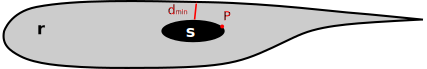
\includegraphics[width=0.45\linewidth]{figures/schematic}
  % \vspace{-30pt}
  \caption{A section view of an object $B$ inside wing $A$ and the minimum distance $d_\text{min}$ between them}
  \label{fig:schematic}
\end{figure}

\qquad When one object encloses another, the minimum distance $d_\text{min}$ between them is greater than zero by some margin.
Therefore, a first approach to a geometric constraint might involve computing $d_\text{min,AB} \geq 0 + \text{tol}$.
We can compute $d_\text{min}$ between two triangulated surfaces by computing the minimum distance between each individual pair of triangles.
The minimum distance between a pair of triangles can be found by a total of fifteen primitive tests between the vertices: six point-triangle tests, and nine line-line tests (Figure~\ref{fig:primitives}). % TODO cite ericson

\begin{equation}
  \label{eq:dmin}
  d_\text{min,AB} = \text{min}(d_{\text{min},ij}) \text{ for each triangle } i, \, j \text{ in surfaces } A, \, B
\end{equation}

\begin{figure}[ht]
  \begin{subfigure}[b]{0.48\textwidth}
    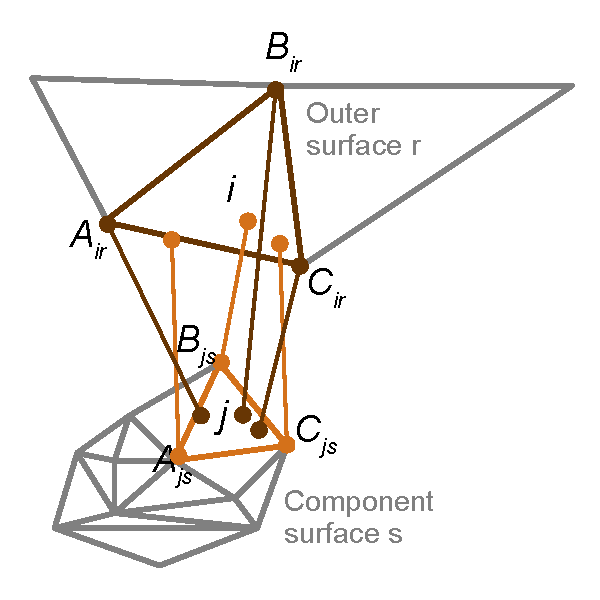
\includegraphics[width=\textwidth]{figures/point-tri.pdf}
    \caption{Six point-tri tests}
    \label{fig:point-tri}
  \end{subfigure}
  \hfill
  \begin{subfigure}[b]{0.48\textwidth}
    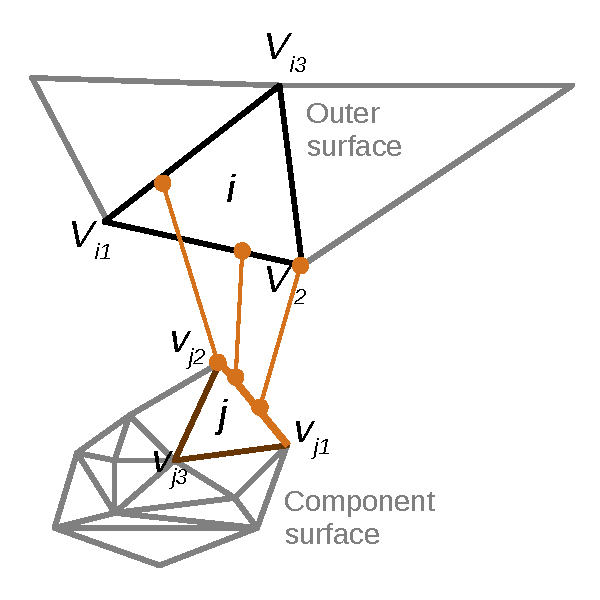
\includegraphics[width=\textwidth]{figures/edge_edge.pdf}
    \caption{Three of nine line-line tests}
    \label{fig:line-line}
  \end{subfigure}
  \caption{Geometric primitive tests between facet $i$ of the outer surface and $j$ of the component}
  \label{fig:primitives}
\end{figure}

\qquad During optimization, the pair of facets comprising the minimum distance can change rapidly, leading to discontinuities in the gradients and poor optimizer performance.
Notionally, we want to gather information not only from the exactly closest triangles, but also from the triangles that are nearly closest.
We can achieve this by using a strategy called constraint aggregation.
I used a function called the Kreisselmeier-Steinhauser (KS) function which essentially provides a conservative estimate of the extremum of a vector.
The computation is as follows:

\begin{equation}
  \label{ks_geom}
  KS_\text{geom}(\textbf{x}) = \frac{1}{\rho} \textrm{ln} \Bigg[\sum_{i,j=1}^{m,n} e^{\rho\big(d_\text{min}\:(\textbf{x})-d_{ij}\:(\textbf{x})\big)}\Bigg] - d_\text{min}\:(\textbf{x}) \leq 0 ,
\end{equation}

where $\textbf{x}$ is a vector of design variables,
$d_{ij}(\textbf{x})$ is the pairwise distance between the $i$th facet of $A$ and $j$th facet of $B$,
$d_{min}(\textbf{x})$ is the minimum distance between $A$ and $B$ at the current design point, and
$\rho$ is a user-controllable constant.

\qquad Last year, I implemented the computation of Equation~\ref{ks_geom} using the Tensorflow framework. % cite tensorflow
Tensorflow is a Python package designed for machine learning, originally developed by Google.
Tensorflow uses a graph representation of a series of array operations and computes a result in a SIMD fashion.
Since many machine learning workflows require gradients for training purposes, Tensorflow natively supports analytic reverse-mode derivatives, making it ideal for use in gradient-based optimization.
Tensorflow also supports heterogeneous computer architectures, including GPU acceleration.
I found that I could run the calculation almost instantaneously on the GPU of my desktop machine. 

\qquad I used my implementation, which I call \emph{geograd} (for ``\emph{geo}metric constraints with \emph{grad}ients''), for several published optimization studies over the last 12 months. %cite scitech, aviation papers
To run the published optimization cases, I used the Texas Advanced Computing Center (TACC) Stampede2 cluster.
Unfortunately, while TACC does have GPU nodes, the geometry calculation is a very small portion of the overall compute cost (which includes expensive, CPU-based fluid dynamics calculations).
Therefore, it did not make economic sense to reserve GPU nodes just for the geometry constraints since it would be idle a large percentage of the time.

\qquad Instead, I used Tensorflow's CPU support and created an optimized, CPU-parallel implementation.
I used the \texttt{mpi4py} package to scatter the computation over all MPI processes, run one Tensorflow call on each process, and gather the results.
I built Tensorflow from source with Intel MKL support and architecture-specific optimizations, including the Intel AVX-512 SIMD extensions.
This confguration provided enough performance for my immediate research needs, but increased the wall time significantly compared to the GPU card on my desktop.
I need to reduce the computation time in order to scale up to more complex optimization problems with more objects to pack inside the airframe.

\qquad Tensorflow's SIMD approach makes it infeasible to use control flow and early exits to reduce the cost of the geometry calculations, which results in a large number of redundant calculations.
I brainstormed several potential approaches which can be used to reduce compute cost, including:
\begin{itemize}
  \item Arranging control flow so that the most likely branches are tested first
  \item Using the minimum instead of the sum of the 15 pairwise primitives for each triangle (reduces the gradient compute cost by 15x)
  \item Using bounding box tests to quickly exclude pairs of facets which are far away from each other and cannot possibly be the minimum distance
\end{itemize}
In order to use these approaches, I need control flow. 
Therefore, I need to drop the Tensorflow SIMD formalism and write my own CPU-optimized implementation in Fortran with Python bindings.
The term project consists of this new Fortran 90 implementation.

\section{Benchmarking Case Description}
\qquad I wanted to isolate performance metrics to the geometry code, yet test the code in a setting representative of an optimization run, so I generated an artificial test problem.
Consider a blended wing body (BWB) aircraft, as pictured in Figure~\ref{fig:bwb-alone}.
We might optimize the shape of this aircraft to minimize drag.
Aircraft also need to hold systems components (such as actuators and hydraulic pumps).
I created a notional football-shaped geometry to represent a generic system component to be packed optimally into the wing and placed it into the right wing root, as pictured in Figure~\ref{fig:bwb-blob}.
We can then compute Equation~\ref{ks_geom} between the aircraft outer shape and the football-shaped inner component to see whether the current layout is feasible.

\begin{figure}[ht]
  \centering
  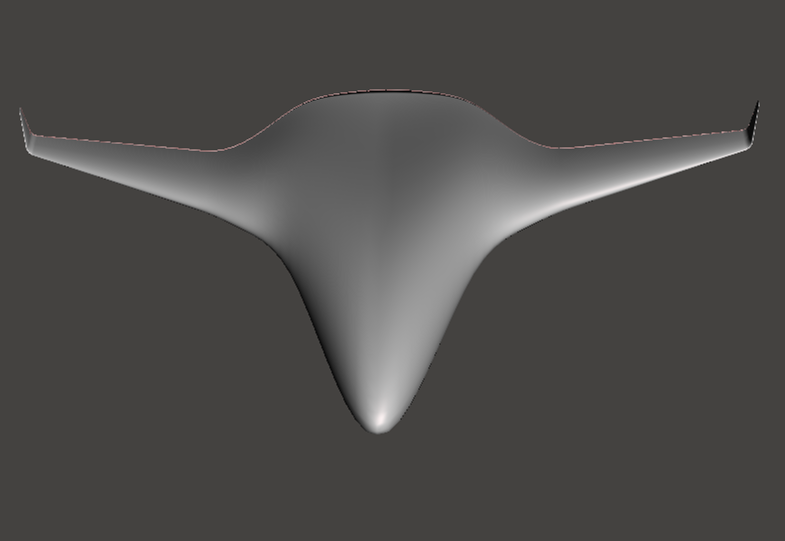
\includegraphics[width=0.66\linewidth]{figures/bwb_alone.png}
  \caption{This blended wing body geometry was used for the test problem}
  \label{fig:bwb-alone}
\end{figure}

\qquad During optimization, the relative positions of the two objects will change. 
Generally, the changes in position will be fairly subtle.
However, to make the test problem as challenging as realistically possible, the component translates from one wing root to the other in 50 equally-spaced increments.
The arrow in Figure~\ref{fig:bwb-blob} shows the path of the component.
The test comprises computing Equation~\ref{ks_geom} 50 times, one at each component position.
I implemented the test as a Python unittest file (\texttt{test\_speed.py} in the repository).
Two timings are obtained; one for analysis only (no gradient), and another with gradients.

\begin{figure}[ht]
  \centering
  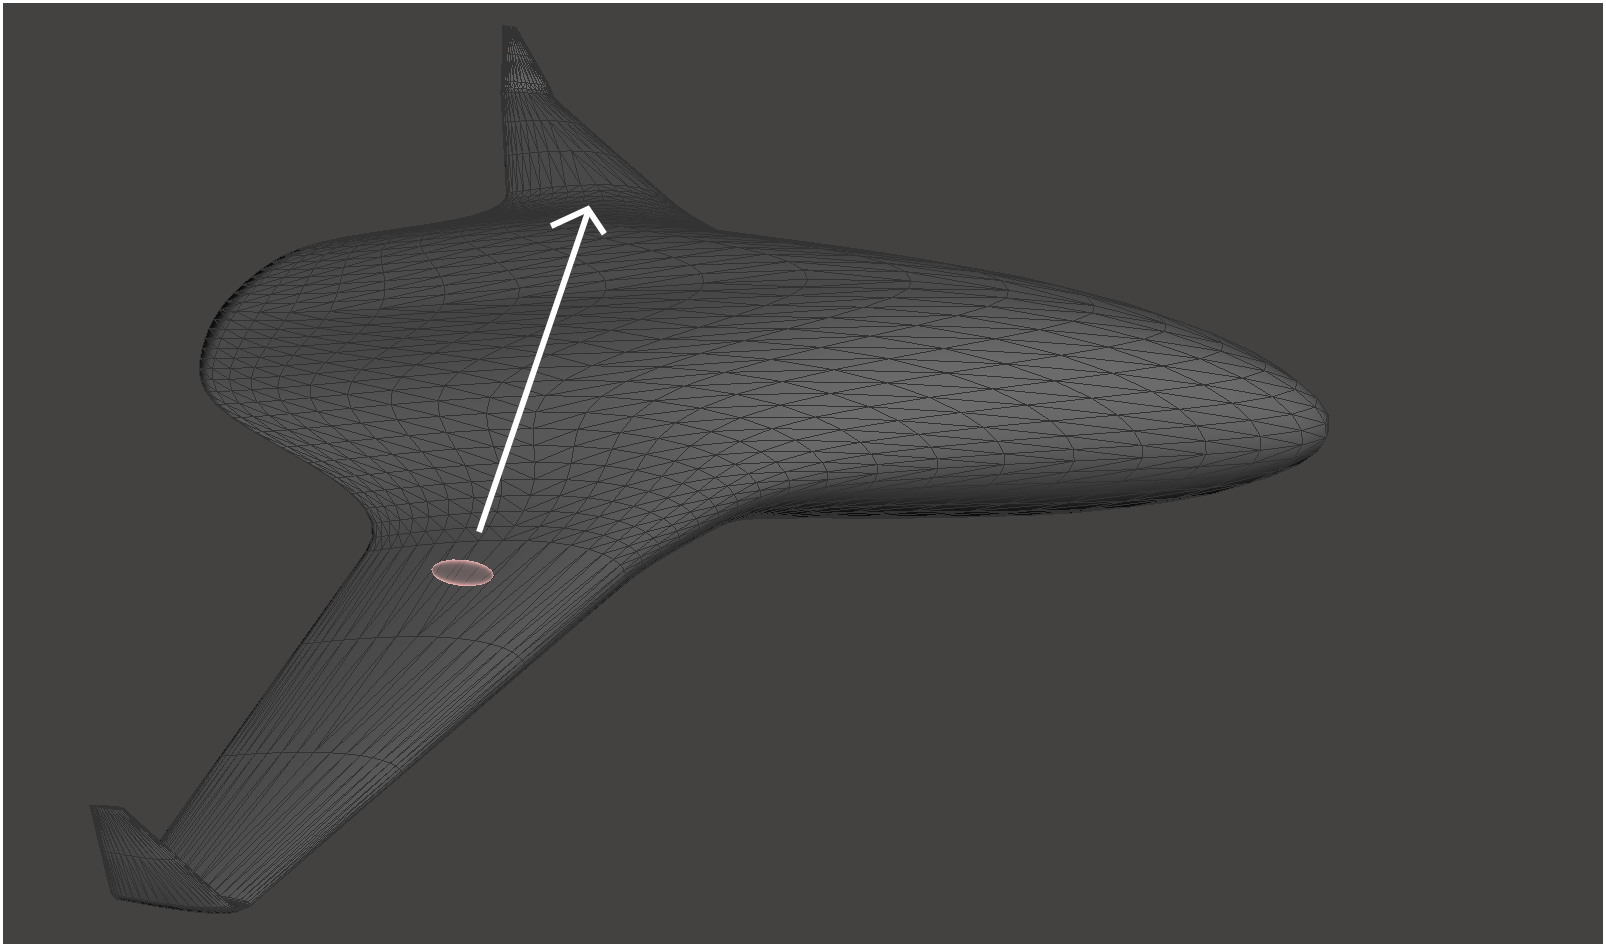
\includegraphics[width=0.80\linewidth]{figures/bwb_With_blob_arrow.png}
  \caption{The component geometry translates from one side of the aircraft to the other in the test problem}
  \label{fig:bwb-blob}
\end{figure}

\section{Baseline Code Development and Verification}
\qquad Because this code will be used to produce published research results, I need to ensure the code is not only fast, but also accurate.
I developed the code in the following general steps:
\begin{itemize}
  \item Writing line-line and point-triangle test primitive subroutines
  \item Algorithmic differentiation of the geometric primitives
  \item Writing the serial KS function subroutine (implementing Equation~\ref{ks_geom})
  \item Creating the Python-Fortran interface
  \item Unit testing of the geometric primitives and KS function
  \item Parallelizing the KS function subroutine
  \item Verification of the derivative output using the complex step methods
\end{itemize}

\subsection{Writing Geometric Primitives}
\qquad I implemented the line-line and point-triangle tests as described in Ericson. % TODO cite ericson
The subroutines, contianed in \texttt{triangles.F90} take four three-dimensional points as input and return the minimum distance.
The sequence of control flow is designed to exit early in some common cases, deferring the least likely paths until as late as possible.
I also developed unit tests using triangles in prescribed configurations to exercise each of the branches of the mathematics.

\subsection{Algorithmic Differentiation of the Primitives}
\qquad We not only need to know the minimum distance result of the primitives; we also need the derivatives with respect to the function inputs.
It is possible to derive this by hand; however, it is much easier to use source code transformation via algorithmic differentiation (AD).
I differentiated the point-triangle and line-line primitive subroutines using the \href{https://www-sop.inria.fr/tropics/tapenade.html}{INRIA Tapenade} software.
There are two modes in AD: forward and reverse (also known as backprop).
I used reverse mode, which requires only one function evaluation to get the derivatives of a single output ($d_{min}$) with respect to all 12 of the inputs (four points, three dimensions each).

\subsection{Assembling the KS Function and Gradients}
\qquad I implemented the loops to compute Equation~\ref{ks_geom} with respect to all of the $m$ facets of an outer surface and $n$ facets of the inner surface.
The subroutine \texttt{compute} takes 8 inputs:

\begin{itemize}
  \item $A_1$, $B_1$, $C_1$: lists of vertices comprising the $m$ triangles of the outer surface
  \item $A_2$, $B_2$, $C_2$: lists of vertices comprising the $n$ triangles of the inner object surface
  \item $d_\text{min,current}$: the minimum distance between the two surfaces at the current design point (this is used to normalize the calculation which improves numerical conditioning)
  \item $\rho$: a user-defined constant which defines how tight the objects can fit next to each other 
\end{itemize}

The subroutine returns:

\begin{itemize}
  \item $KS$: the constraint described in Equation~\ref{ks_geom}
  \item $d_\text{min}$: minimum distance between the two surfaces
\end{itemize}

I also wrote a function \texttt{compute\_derivs} which additionally computes the following derivatives with respect to the surface mesh points (all $m$ by 3 arrays):

\begin{equation}
  \frac{dKS}{d\textbf{A}_1} \, \, \, \, \, \, \frac{dKS}{d\textbf{B}_1} \, \, \, \, \, \, \frac{dKS}{d\textbf{C}_1} 
\end{equation}

and the following derivatives with respect to the object mesh points (all $n$ by 3 arrays):

\begin{equation}
  \frac{dKS}{d\textbf{A}_2} \, \, \, \, \, \, \frac{dKS}{d\textbf{B}_2} \, \, \, \, \, \, \frac{dKS}{d\textbf{C}_2} 
\end{equation}

Differentiating top-level code, particularly when it involves dynamically-allocated arrays or MPI calls, can be very inefficient.
Therefore, I differentiated Equation~\ref{ks_geom} by hand using the AD results for the geometric primitives.
% TODO write down the expression
Since the entries of the derivatives depend on both local information as well as the global summation across all the facet pairs, the overall computation is not embarassingly parallel.
However, the amount of communication required is fairly low (a single partial sum is Allgathered from all processes) in between two separate double $ij$ loops.
There is also no stencil-type calculation where offsets from $ij$ are used, meaning that an owner-computes approach will be fine.



\end{document}
